\section{Bayesian Approach Introduction} 

As discussed in \cref{sec:back_optimization} previous work has explored learning
from qualitative feedback such as preferences in order to circumvent defining
objective functions. Also, Bayesian optimization has been proposed to reduce the
number of experiments required to solve optimize problems. In this first half of
this chapter, we present a new optimization algorithm, Predictive Entropy Search
with Preferences (PES-P), that combines these two ideas. We adapt an acquisition
function previously proposed for interval scale feedback to the preference
feedback case. This acquisition function seeks a pair of parameters for which a
preference will maximally reduce the entropy of the distribution of objective
function optima. To test the algorithm, we compare in simulation the
performance of the proposed optimization method against the expected improvement
method (EI) and uniform random sampling via Latin hypercubes (LH) for two
classes of examples: optimizing randomly generated objective functions and
tuning the control parameters of simulated dynamical systems. 

\subsection{Learning from Preferences}

To learn latent objective functions from preferences, we rely on the method
developed by \citeauthor{chu2005preference}~\citep{chu2005preference}, briefly
reviewed here.  The method considers a training dataset $D_n$ of $n$ preferences
between pairs of points, $\{x_1^\tn{a} \succ x_1^\tn{b}, \ldots, x_k^\tn{a}
\succ x_k^\tn{b}, \ldots, x_n^\tn{a} \succ x_n^\tn{b}\}$. These points can, for
instance, represent control policy parameters. From the dataset, the method
finds a posterior distribution of latent objective functions $\vecf{f}$,
\begin{align}
    \prob{\vecf{f}|D_n} = \frac{\prob{D_n|\vecf{f}}
        \prob{\vecf{f}}}{\prob{D_n}}.
    \label{eq:bayes_rule}
\end{align}
where $\vecf{f} = [f(x_1^\tn{a}), f(x_1^\tn{b}), \ldots, f(x_n^\tn{a}),
f(x_n^\tn{b})]^T$. First, the method assumes that the prior distribution of
objective functions is a zero-mean \emph{Gaussian process} (GP),
$\prob{\vecf{f}} = \mathcal{N}(0, \Sigma)$. An appropriate kernel, $\Sigma_{i,j}
= \func{k}(x_i,x_j)$, describes the elements of the covariance matrix $\Sigma$.
(See~\citep{williams2006gaussian} for a full description of GPs.) Second,
$\prob{D_n|\vecf{f}}$ is the overall likelihood of preferences in the
dataset given specific reward function values and is modeled as the product of
the likelihood of each independent preference in the dataset,
\begin{align}
    \prob{D_n|\vecf{f}} &= \prod_{k=1}^n \prob{x_k^\tn{a} \succ x_k^\tn{b} 
            | f(x_k^\tn{a}), f(x_k^\tn{b})} 
        = \prod_{k=1}^n \Phi(q_k),
    \label{eq:likelihood}
\end{align}
where $\prob{x_k^\tn{a} \succ x_k^\tn{b} | f(x_k^\tn{a}), f(x_k^\tn{b})}$ is the
probability of a preference if Gaussian noise with variance $\sigma^2$ corrupts
the function values, $\Phi(\cdot)$ is the cumulative distribution function of a
normal distribution, and $q_k = \frac{f(x_k^\tn{a}) - f(x_k^\tn{b})}{\sqrt{2}
\sigma}$.  In essence, the likelihood model increases the certainty of a
preference between $x_k^\tn{a}$ and $x_k^\tn{b}$ as the difference between
$f(x_k^\tn{a})$ and $f(x_k^\tn{b})$ widens. 

To obtain the posterior distribution $\prob{\vecf{f}|D_n}$ the method
approximates \cref{eq:bayes_rule} with a Gaussian distribution. As a result, the
predictive distribution (subscript p) of the objective function at test points,
$\vecf{f}[\tn{t}]$, is also Gaussian, $\prob{\vecf{f}[\tn{t}] | D_n} =
\mathcal{N} \left( \mu_\tn{p}, \Sigma_\tn{p} \right)$. Finally, the predictive
distribution of a preference between two points $x^\tn{a}$ and $x^\tn{b}$ is 
\begin{align} 
    \prob{x^\tn{a} \succ x^\tn{b} |D_n} 
    &=\hspace{-2pt}\int \prob{x^\tn{a} \succ x^\tn{b}|\vecf{f}[\tn{t}],D_n}
    \prob{\vecf{f}[\tn{t}]| D_n} \tn{d} \vecf{f}[\tn{t}] 
        \label{eq:prob_of_pref}\\
    &= \Phi \left(\frac{\mu^\tn{a} - \mu^\tn{b}}{\sigma_\tn{p}} \right),
        \label{eq:p_pref} \\ 
    \sigma_\tn{p}^2 &= 2\sigma^2 + \Sigma_\tn{p}^\tn{aa} + \Sigma_\tn{p}^\tn{bb}
        - \Sigma_\tn{p}^\tn{ab} - \Sigma_\tn{p}^\tn{ba}.
\end{align}

\Cref{fig:pes_plot}a provides an example of how the method estimates a
ground-truth objective function shown in purple. The blue line and shaded area
show the mean and standard deviation of the posterior distribution of objective
functions, $\prob{\vecf{f}_\tn{t}|D_n}$, after two preference queries between
pairs of parameters (orange, higher is preferred over lower value). The queries
have the effect of lifting the estimated objective function close to preferred
points and pushing it down close to unpreferred points, approximating the true
objective function over time.

\subsection{Active Learning for Optimization}
Learning from preferences describes how to find a distribution of objective
functions given a dataset of comparisons. The question now becomes how to
efficiently solicit preferences from the user. As our main goal is to find the
optimal parameters $x^*$, we should forgo modeling the objective function
accurately in all parameter regions and instead focus on regions where the
objective might be high. Bayesian optimization addresses this problem with an
acquisition function that helps to efficiently sample training data.
\begin{marginfigure}
    \centering
    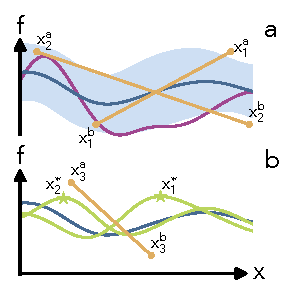
\includegraphics[width=\linewidth]{pes_plot}
    \caption{Learning from preferences. (a) Mean and standard deviation of
    $\prob{\vecf{f}[\tn{t}]|D_n}$ (blue) after two preferences queries (orange)
    from the true objective function (purple). (b) Mean of
    $\prob{\vecf{f}[\tn{t}]|D_n}$ (blue) and means of
    $\prob{\vecf{f}[\tn{t}]|D_n, x_m^*}$ (green) for two samples of $x_m^*$.
    PES-P queries a new comparison (orange) for which the preference is
    currently uncertain, but on average is certain after conditioning on all
    $x_m^*$.}\label{fig:pes_plot}
\end{marginfigure}

One such acquisition function is the expected improvement, which has been used
both in the context of preference feedback~\citep{eric2008active} and interval
scale feedback~\citep{jones1998efficient},
\begin{equation}
    \func{EI}{x} = (\mu^* - \mu(x))\Phi(d) + s(x)\phi(d),
    \label{eq:expected_improvement}
\end{equation}
where $d = (\mu^* - \mu(x))/s(x)$, $\mu^*$ is the mean of the current estimate
of the optimum, and $\mu(x)$ and $s(x)$ are the mean and standard deviation of
the objective of a new point $x$, respectively. As an alternative, for interval
scale feedback,~\citep{hennig2012entropy} and~\citep{hernandez2014predictive}
proposed acquisition functions that seek to reduce the uncertainty in the
distribution of objective function optima, measured in terms of the differential
entropy. For example, the Predictive Entropy Search acquisition
function~\citep{hernandez2014predictive} seeks a point $x$ that is expected to
reduce the entropy of the distribution of optima $x^*$ after observing its value
$y$,
\begin{align}
    \alpha_n \left(x \right) = \funcsb{H}{\prob{x^*|D_n}} 
        - \funcsb{E}[\prob{y|x, D_n}]{\funcsb{H}{\prob{x^*|y, x, D_n}}},
    \label{eq:pes_interval_scale}
\end{align}
where $\funcsb{H}{\prob{x}} = - \int \prob{x} \log \prob{x} \tn{d} x$
is the differential entropy. The authors of these methods have shown they can
outperform EI\@. 
